\section{Simulations}\label{sec:simulations}

There are two main randomized simulation scenarios inside simulation module 
(module described in \ref{subsec:simulations-architecture}).
First simulation is designed to be static.
It creates only one execution plan
and then it shut downs.
The second simulation reflects the presumed production environment
and is described in the figure \ref{fig:simulation-process}.

\begin{figure}[ht] 
	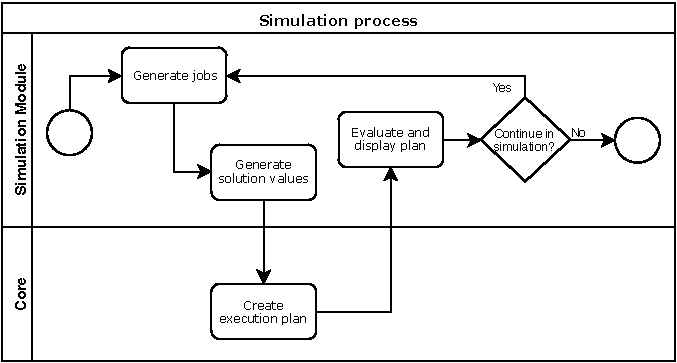
\includegraphics[width=\textwidth]{i_simulation_process.pdf} 
	\centering
	\caption{Simulation process}
	\label{fig:simulation-process}
\end{figure}

\begin{itemize}
  \item \textbf{Generate jobs} - simulation randomly create new optimization jobs, 
  which should be scheduled by the core.
  It also generates their scheduling parameters.
  \item \textbf{Generate solution values} - simulation uses the solution values functions,
  generated by the TASP (\ref{subsubsec:tasp}) algorithm as described in section \ref{sec:optimization-algorithms-data}.
  The data files are randomly assigned to the particular jobs, 
  therefore each job represents unique TASP instance
  and has unique solution value during time.
  \item \textbf{Create execution plan} - simulation executes plan creation by calling the core API.
  The process of plan creation is described in section \ref{sec:olb-algorithm}.
  \item \textbf{Evaluate and display plan} - simulation engine uses evaluator to check for the constraint violations
  and then prints the result into the log.
  It also prints the text representation of the plan into the standard output. 
  An example of such plan in text representation can be seen in listing \ref{lst:data-example}.
\end{itemize}

\subsection{Simulation output}\label{subsec:simulation-output}

Simulation's output (produced execution plan) is printed to standard output.
Data displayed in listing~\ref{lst:data-example} are an exact output produced by the simulation with 5 jobs being scheduled at once.
The optimization jobs,
which were scheduled in the listing~\ref{lst:data-example},
have their parameters displayed in the table~\ref{table:jobs-parameters}

\begin{table}[ht]
	\centering
	\caption{Table with the input and output parameters of the jobs}
	\begin{tabular}{|c|c c c c c|} 
		\hline
		Job ID   & 0      & 1     & 2     & 3     & 4     \\
		\hline\hline
		$D^{j}$  & 284    & 161   & 373   & 271   & 129   \\
		\hline
		$P^{j}$  & 757    & 42    & 73    & 51    & 29    \\
		\hline
		$T^{j}$ & 180    & 120   & 360   & 240   & 120   \\
		\hline
    $C^{j}$     & 131.20 & 24.36 & 65.08 & 39.16 & 28.48 \\
    \hline
	\end{tabular}
	\label{table:jobs-parameters}
\end{table}

The variables $D,P,T$ and $C$ are defined in section \ref{sec:formal-definition}
and represents following data related to the one job.
\begin{itemize}
  \item $D^{j}$ - maximal duration of the job execution which cannot be exceeded
  \item $P^{j}$ - maximal used resources cost per job,
  or in other words highest possible price paid for the job execution which cannot be exceeded
	\item $T^{j}$ - time taken, duration of the actual job execution
	\item $C^{j}$ - resource costs, how much money was actually paid for the job execution
\end{itemize}

The following data output is result of the first scheduling window 
(how does the load balancing algorithm work is described in section \ref{sec:olb-algorithm}).

\noindent
\begin{minipage}{\textwidth}
  \begin{lstlisting}[caption={Simulation data output},label={lst:data-example},language=Kotlin]
    0 iteration:
                Times:||  0| 60|120|180|240|300|360|
    ----------------- || --|---|---|---|---|---|---|
        Cost: 1 + 0.02||  2|  2|  4|  3|  3|  2|  2|
        Cost: 1 + 0.02||  2|  2|  4|  3|  3|  2|  2|
        Cost: 1 + 0.02||  2|  2|  4|  3|  3|  2|  2|
        Cost: 1 + 0.02||  3|  4|  4|  3|  3|  2|  2|
        Cost: 1 + 0.02||  4|  4|  4|  3|  3|  2|  2|

      Cost: 1.5 + 0.02||  1|  1|  1|  2|   |   |   |
      Cost: 1.5 + 0.02||  1|  1|  1|  2|   |   |   |

     Cost: 10.0 + 0.05||  0|  0|  0|  0|   |   |   |
     Cost: 10.0 + 0.05||  0|  0|  0|  0|   |   |   |

    Total plan cost: CostImpl(value=264.587)$
  \end{lstlisting}  
\end{minipage}

\bigskip \noindent
\inlinecode{Times} axis shows time units ($t$ value described in section \ref{sec:formal-definition}) in seconds.
Second, vertical axis, visualizes resources.
Name, \inlinecode{Cost: 1 + 0.02} is name of the resources provider (explained in section \ref{subsec:formalized-definition-representation}),
and each line is one usage unit - meaning that it could be one physical core or for example percentage of shared processor.
In implementation, this value is referred as CPU core,
but in fact, it is dimensionless value expressing usage of some system resources.

Each cell contains either number or is empty.
Number is job ID and indicates, that this resource is allocated to job with displayed ID.
This is effectively $^{r}x_{t}^{j}$ value explained in section \ref{subsec:variables-definition}.

Total plan cost is sum of all particular costs of all jobs - their resources allocations.
Therefore this is the cost of the created execution plan.